
\subsection{Intelligent attack mitigation}
\label{sec:intelligent mitigating}

%While the Interest limit is the key building block to suppress mechanisms of the Interest flooding attack, legitimate Interests need to be somehow prioritized and malicious Interests need to be somehow penalized in order to completely suppress the attack.
%That is, instead of processing Interests always based on the first-in-first-serve rule, NDN routers need some basis to treat the incoming Interests differently.
%Thus, the primary task in bringing intelligence to the Interest flooding attack mitigation is to proactively distinguish between legitimate and malicious Interests.

In order to distinguish between legitimate and malicious Interests, we leverage another unique feature of  NDN architecture---guaranteed symmetric flow of Interest and Data packets. Since a Data packet takes the reverse path of the corresponding Interest packet, a router is guarateed to see if an Interest it forwarded resulted in a matching Data packet. The only exception being if Interest/Data packets were lost along the way due to congestion in the network.
Therefore, intermediate routers can classify all Interests that result in matching Data as legitimate, while the ones that timed out can be marked as malicious.\footnote{Recall that in order to maximize effect of the Interest flooding attack, an adversary expresses a large volume of junk Interests (see Section~\ref{sec:interest flooding}).}  
%Implications of other types of attacks are discussed in Section~\ref{sec:discussion}.}

This timeout-based differentiation method is reactive in nature: one cannot determine in advance if an Interest will result in a timeout or Data being retrieved. However, routers can proactively maintain up-to-date statistics of Interest satisfaction ratios (number of forwarded versus number of satisfied Interests), and use this statistic to determine whether an incoming Interest must be forwarded or dropped. For example, maintaining independent Interest satisfaction ratio statistics for each incoming interface is sufficient to estimate whether an Interest received from a neighbor connected to this interface will result in a Data packet or a timeout. Statistics can also be kept at finer granularities such as per outgoing interface, per name prefix, etc. that can further improve the estimates. A router's goal should be to penalize malicious Interests as soon as possible---negative statistics should be allowed to build up fast, while positive statistics should not be allowed to deteriorate too quickly. We use the standard exponentially weighted moving average, performed once a second with $\alpha$ coefficient $e^{-1/30}$, approximately corresponding to a 30-second averaging window to achieve the above goal.

%Choosing the right balance between these contradictory requirements is a challenge and we explore this topic further  in the evaluation section.  %{\color{red} \it Priya: we should address the one that works best such as exponentially weighted moving average in eval section - it doesn't belong %here.} 

%The devil is always in the details.
%From the one hand, such statistics needs to start penalizing adversaries as soon as possible (i.e., negative stats should build up fast).
%On the other hand, the positive statistics should not deteriorate too fast (i.e., positive stats should be relatively long-term).
%Our preliminary experiments showed that the standard exponentially weighted moving average, performed once a second with $\alpha$ coefficient $e^{-1/30}$, approximately corresponding to a 30-second averaging window, provides a good balance between the two contradictory requirements.

% \subsubsection{\textbf{Data plane performance tracking}}
% \label{sec:stats}

% Note that there is a condition (line 6 in Pseudocode~\ref{alg:probabilistic model}) to check if there is a valid statistics point.
% This condition is extremely important, because it first provides a basis to distinguish between known facts (i.e., good or bad satisfaction ratio for the incoming interface) and unknown facts (e.g., the first time an Interests arrives on the interfaces).
% Second, it gives an opportunity to recover from a bad history (history of unsatisfied Interests) after malicious Interests are ceased to flow in.
% Essentially, this recovery relies on statistics module to perform time-based invalidation of historical data (timely, but not too quickly\footnote{Otherwise, attackers may send short bursts of malicious Interests, successfully avoiding differential Interest treatment}).


Pseudocode~\ref{algo:interest stats} formally defines how statistics can be generated for  each incoming interface. Note that in order to ensure decaying of relative statistics (e.g., ratio between the number of unsatisfied and forwarded Interest), only unsatisfied statistics needs to be exponentially smoothed (lines 23--26).  

\floatname{algorithm}{Pseudocode}

%%%%%%%%%%%%%%%%%%%%%%%%%%%%%%
%%%%%%%%%%%%%%%%%%%%%%%%%%%%%%
%%%%%%%%%%%%%%%%%%%%%%%%%%%%%%

\begin{algorithm}[h]
\footnotesize
\caption{\small Interest satisfaction statistics}
\label{algo:interest stats}
\begin{algorithmic}[1]

\For{\textbf{each} interface \textbf{if}}
    \State $F_{if} \leftarrow 0$ \Comment{forwarded Interests from interface \textbf{if}}
    \State $\hat F_{if} \leftarrow 0$ \Comment{averaged value of $F_{if}$}

    \State $U_{if} \leftarrow 0$ \Comment{unsatisfied Interests from interface \textbf{if}}
    \State $\hat U_{if} \leftarrow 0$ \Comment{averaged value of $U_{if}$}
\EndFor

\vspace{0.1cm}
\Function{OutInterest}{Interest \textbf{i}, InInterface \textbf{in}}
  \State $F_{in} \leftarrow F_{in} + 1$
  \State record \textbf{\emph{in}} in the list of incoming interfaces for \textbf{\emph{i}}
\EndFunction

\vspace{0.1cm}
\Function{InterestTimeout}{Interest \textbf{i}}
    \State lookup the list of incoming interfaces for \textbf{\emph{i}}

    \For{\textbf{each} interface \textbf{if} in the list}
        \State $U_{if} \leftarrow U_{if} + 1$
    \EndFor
\EndFunction

\vspace{0.1cm}

\State {} \Comment{\textit{Exponentially weighted moving average smoothing}}
\Function{EWMA}{} \Comment{Every second}
\State $\alpha \leftarrow e^{-1.0/30.0}$  %\Comment{$\approx$ 30~sec average}

\For{\textbf{each} interface \textbf{if}}
    \State $\hat U_{if} \leftarrow \alpha \cdot \hat U_{if} + (1 - \alpha) \cdot U_{if}$ 
    \State $U_{if} \leftarrow 0$ 

    \If{$F_{if} > 0$} \Comment{To ensure decaying of ratio $U_{if}/F_{if}$}
        \State $\hat F_{if} \leftarrow \alpha \cdot \hat F_{if} + (1 - \alpha) \cdot I_{if}$ 
        \State $F_{if} \leftarrow 0$ \Comment{Reset counters}
    \EndIf
\EndFor

\EndFunction

\end{algorithmic}
\end{algorithm}


Fig.~\ref{fig:ratio example} illustrates the resulting dynamics of the statistic during and after an Interest flooding attack. The attack duration is from 10 to 70~seconds. Prior to start of the attack, the percentage of unsatisfied Interests is zero.  
The statistics build up rapidly as soon as Interests start to time out, which happens approximately one second after the start of the attack.\footnote{Again, we are assuming that Interests are admitted for a maximum period one second.}
For the duration of the attack (10--70~seconds), the percentage of unsatisfied Interests is close to 100\%: 
when the ratio is close to 100\%, routers drop all incoming Interests, resulting in decaying of the statistics until a new Interest is admitted, which eventually brings statistics back near 100\% point.
Finally, the ratio exponentially decays after the attack ceases.

\begin{figure}[htbp]
  \centering
  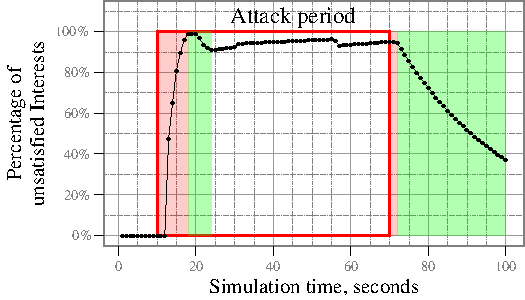
\includegraphics[scale=0.8]{limits}
  \caption{Dynamics of the unsatisfied Interests statistics on gateway's interface towards the attacker}
  \label{fig:ratio example}
\end{figure}

%%%%%%%%%%%%%%%%%%%%%%%
%%%%%%%%%%%%%%%%%%%%%%%
%%%%%%%%%%%%%%%%%%%%%%%

\subsubsection{\textbf{Satisfaction-based Interest acceptance}}
\label{sec:probabilistic}

Having successfully implemented a technique to gather statistics on Interest satisfaction ratios, our next challenge is in using this rotio to penalize malicious Interests. A straightforward method to achieve this enforcement is to use the Interest satisfaction ratio as a direct probability for accepting (forwarding) or rejecting an incoming Interest (see Pseudocode~\ref{alg:probabilistic model}).
%Apart from the Interest satisfaction statistics generation, there is a question how this statistics can be used to actually enforce prioritization and penalizing of Interests.


\floatname{algorithm}{Pseudocode}

%%%%%%%%%%%%%%%%%%%%%%%%%%%%%%
%%%%%%%%%%%%%%%%%%%%%%%%%%%%%%
%%%%%%%%%%%%%%%%%%%%%%%%%%%%%%

\begin{algorithm}[h]
\footnotesize
\caption{\small Satisfaction-based Interest acceptance}
\label{alg:probabilistic model}
\begin{algorithmic}[1]
\State{} \Comment{Same init, InData and Timeout functions as in Pseudocode~\ref{alg:queuing}}

\vspace{0.1cm}
\Function{OutInterest}{Interest \textbf{i}, InInterface \textbf{in}, OutInterface \textbf{out}}

    \State{} \Comment{Use uniform probability distribution model $P(X)$}
    \State{} \Comment{$P(X) : \forall x \in [0,1] \Rightarrow P(x) = x$}
    
    \If{$F_{in} > \theta $} \Comment{At least some Interests were forwarded before}
        \State $s \leftarrow (1 - U_{in} / F_{in})$
        \State Drop interest with probability $P(s)$
    \EndIf

    \State{forward the Interest, subjecting to token bucket limits}
\EndFunction

\end{algorithmic}
\end{algorithm}

Parameter $\theta$ on line 5 of the Pseudocode~\ref{alg:probabilistic model} ensures that the probabilistic model is not enforced when the volume of Interests arriving at a particular interface is small. This step is critical---while we want to drop Interests from attackers, we also want to provide an opportunity for legitimate users to regain their share of resources after temporary Data delivery failures.

A drawback of the satisfaction-based Interest acceptance method is that each router on the path makes an independent decision on whether to forward or drop the Interest. 
As a result of these independent decisions,  the probability of legitimate Interests being forwarded decreases rapidly as the number of hops between the content requester and producer grows; worsening the Interest satisfaction statistics and resulting in further drops.
In example on Fig.~\ref{fig:flooding example}, the router A observes 50\% satisfaction rate for \texttt{eth1} and 0\% rate for \texttt{eth0}. 
At the same time, router B observes a 30\% satisfaction rate for its \texttt{eth0} interface.
Next time a legitimate Interest arrives at router A, it has a 50\% chance of being forwarded further, and if forwarded, it has only a $50\% \times 30\% = 15\%$ probability of being forwarded further towards the Data producer. With each increasing hop in the network, the probability of being forwarded to the next hop decreases significantly. 
One way to prevent this overreaction and unfair penalization is to ensure that the decision taken at each router on whether to forward or drop the Interest is not independent of the decision taken at preceding routers. An explicit notification such as a gossip protocol between neighboring NDN routers that specifies the volume of Interests each router is willing to forward will likely address this issue. We leave the implementation and evaluation of a gossip protocol to future work.
%{\color{red}Alex: we should state that it is out of scope of the paper to evaluate this issue}

%%%%%%%%%%%%%%%%%%%%%%%
%%%%%%%%%%%%%%%%%%%%%%%
%%%%%%%%%%%%%%%%%%%%%%%

\subsubsection{\textbf{Satisfaction-based pushback}}
\label{sec:dynamic limits}

% Differential treatment of Interests received from different interfaces can be achieved in a more elegant way, without reverting to probabilistic methods.

The previous algorithm---the satisfaction-based Interest acceptance---divides the available forwarding tokens among all interfaces in proportion to their Interest satisfaction ratios.
% Given the drawbacks of this algorithm, the same effect can be achieved without relying on probabilistic models. 
An alternate algorithm for proportional token distribution without overreaction is to enable and enforce explicit Interest limit for each incoming interface, where the value of the limit depends directly on the interface's Interest satisfaction ratio.
Routers need to announce these limits to their downstream neighbors, ensuring that any Interest forwarded from the downstream router is allowed to get through, resulting in genuine Interest satisfaction statistics.

The formal definition of the satisfaction-based pushback algorithm is presented in Pseudocode~\ref{alg:dynamic limits}, while Fig.~\ref{fig:dynamic limits example} illustrates how the algorithm will work in our example in Fig.~\ref{fig:flooding example}.
Assuming an initial token bucket limit $L=10$ and the current satisfaction ratio for router A is 50\% for \texttt{eth1} and 0\% for \texttt{eth0}, and for router B the ratio is 30\% for \texttt{eth0}, each node will set and announce the following  incoming interface limit $L'$: 
\begin{enumerate}
\item router B will set and announce the incoming interface limit $L'=3$;
\item router A, after receiving announcement from B will readjust its incoming interface limits to $L'_{eth1} = 1.5$ and $L'_{eth0} = 0$; and
\item both legitimate users and adversaries may either obey or ignore the announced limit, which will be in any case enforced by router A.
\end{enumerate}


\begin{figure}[htbp]
  \centering
  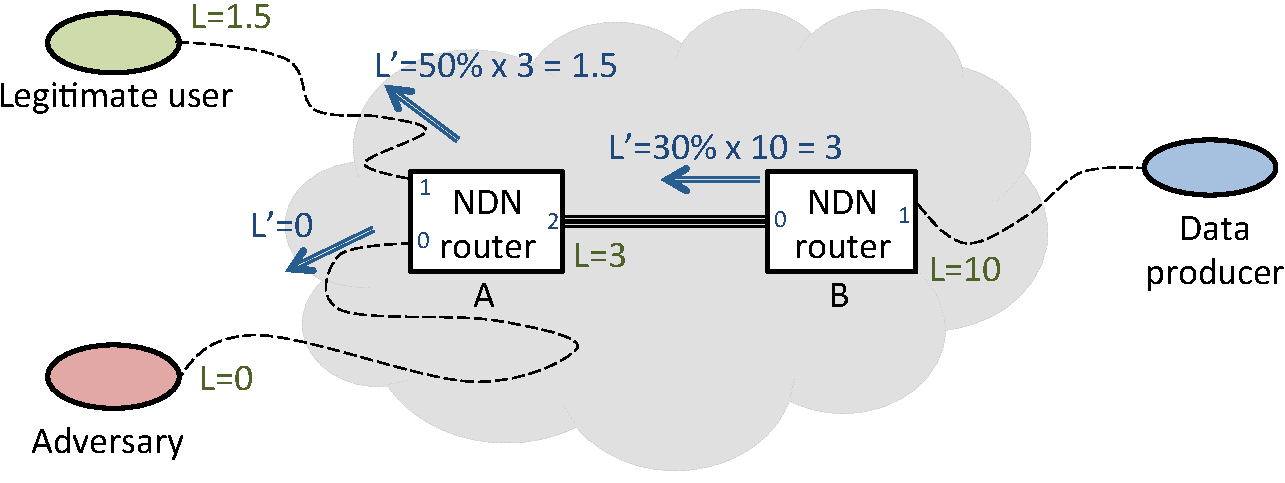
\includegraphics[scale=0.3]{dynamic-limits}
  \caption{Satisfaction-based pushback example
%: routers explicitly tell neighbors how many Interest packets they can deliver to the Data producer%
}
  \label{fig:dynamic limits example}
\end{figure}


\floatname{algorithm}{Pseudocode}

%%%%%%%%%%%%%%%%%%%%%%%%%%%%%%
%%%%%%%%%%%%%%%%%%%%%%%%%%%%%%
%%%%%%%%%%%%%%%%%%%%%%%%%%%%%%
{ 
\begin{algorithm}[h]
\footnotesize
\caption{\small Satisfaction-based pushback}
\label{alg:dynamic limits}
\begin{algorithmic}[1]
% \State{}\Comment{Same initialization, InData and Timeout functions as in Pseudocode~\ref{alg:queuing}}
\State{} \Comment{Same init, InData and Timeout functions as in Pseudocode~\ref{alg:queuing}}
\vspace{0.1cm}
\State{$\forall f \in \mathrm{interfaces} : L'_{f} \leftarrow L_{f}$} \Comment{Per-incoming interface Interest limit} 

\vspace{0.1cm}

\State{} \Comment{\textit{Announcement from the neighbor}}
\Function{InLimits}{InInterface $in$, Limit $L'$}
    \State $L_{in} \leftarrow L'$
\EndFunction

\vspace{0.1cm}

\Function{AnnounceLimits}{} \Comment{\textit{E.g., every second}}
\For{\textbf{each} outgoing interface $out$}

   \For{\textbf{each} incoming interface $in$}
        \State $L'_{in}= {L_{out}} \times (1 - U_{in}/F_{in})$
        \State AnnounceLimit($in$, $L'_{in}$)
   \EndFor

\EndFor
\EndFunction

\end{algorithmic}
\end{algorithm}


The zero limit for the adversary's link implies that  router A is temporarily not willing to accept any Interests from this interface until the statistics decay to the appropriate level (recall Fig.~\ref{fig:ratio example}).
At the next iteration of the satisfaction-based pushback algorithm, the legitimate user will be able to gradually improve the statistics on both routers A and B as all Interests from the user will get through and will return Data, eventually resulting in a full allowance ($L'=L=10$) in the links between the routers A and B, and the user and router A.

We note that while in the description of the satisfaction-based pushback algorithm we explicitly used ``outgoing'' and ``incoming'' interfaces,  all interfaces can be both incoming and outgoing.
Thus, it may not be entirely clear which outgoing limit $L_{out}$ (line 10 in the algorithm) should be used to calculate the incoming limit $L_{in}$.
To overcome this problem, in our actual implementation we enforced separate incoming/outgoing interface limits for each individual FIB entry.
That is, for each FIB entry we set a separate Interest limit for each incoming interface (${L'}_{in}^{fib}$) based on a sum of FIB entry limits for each outgoing interface $L=\sum{L_{out}^{fib}}$.


Both satisfaction-based Interest acceptance and satisfaction-based pushback algorithms are forms of a well-known push-back mechanism~\cite{Pushback}, but with several core differences. 
First, we are suppressing (pushing back) unwanted requests for Data, not actual Data itself.
Second, differentiating between good and bad Interests is based on the traffic symmetry principle of NDN.
% Alex: I'm not entirely sure about this point... 
Finally, both intelligent attack mitigation algorithms can be deployed at all times without degrading network performance even when there are no active attackers. 

%%% Local Variables: 
%%% mode: latex
%%% TeX-master: "paper"
%%% End: 


